\chapter{Introduction}

\blindtext

Another source of inspiration, as you may have noticed, is the
\href{https://github.com/Tufte-LaTeX/tufte-latex}{Tufte-Latex Class}.
The fact that the design is similar is due to the fact that it is very
difficult to improve something which is already so good. However, I like
to think that this class is more flexible than Tufte-Latex. For
instance, I have tried to use only standard packages and to implement as
little as possible from scratch;\sidenote{This also means that
understanding and contributing to the class development is made easier.
Indeed, many things still need to be improved, so if you are interested,
check out the repository on github!} therefore, it should be pretty easy
to customise anything, provided that you read the documentation of the
package that provides that feature \cite{Battle2014}.


\begin{marginfigure}[+1.5cm]
	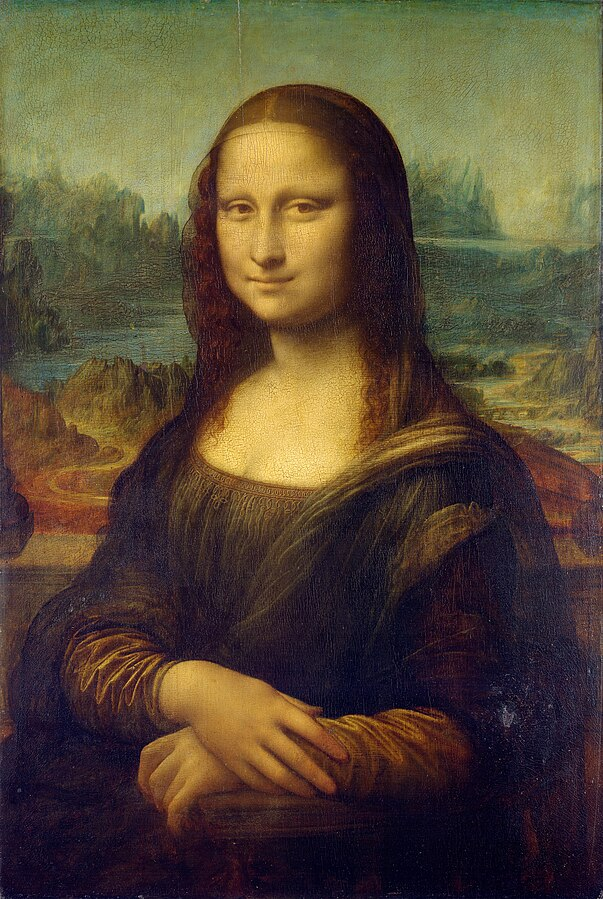
\includegraphics{monalisa.jpg}
	\caption[The Mona Lisa]{The Mona Lisa.\\
	\url{https://commons.wikimedia.org/wiki/File:Mona_Lisa,_by_Leonardo_da_Vinci,_from_C2RMF_retouched.jpg}}
	\labfig{marginmonalisa}
\end{marginfigure}

